\section{Auswertung}
\label{sec:Auswertung}
%Hier kannst du ja noch einen Satz schreiben, wenn du möchtest xD

Da es sich beim Radioaktivenzerfall um eine Poissonverteilung handelt, ist die Abweichung durch die Wurzel des Wertes gegeben

\begin{equation}
    \Delta N = \sqrt{N} \, .
\end{equation}
\subsection{Strahler}
\label{subsec:gammaStrahler}

Die zunächst durchgeführte Nullmessung hat die folgenden Werte ergeben:
\begin{equation*}
    t  = 900 \, \unit{\second} \,
\end{equation*}
\begin{equation*}
    N_0  = 845 \pm 29
\end{equation*}
und

\begin{equation*}
    A_0 = (0.94 \pm 0.032)\dfrac{1}{\unit{\second}} \, .
\end{equation*}

In der \autoref{tab:gammablei} sind die Messdaten der ersten Messreihe angegeben.

\begin{table}[H]
    \centering
    \caption{Messwerte zum $\gamma$-Strahler mit Bleiabschirmung.}
    \label{tab:gammablei}
    \sisetup{table-format=1.2}
    \begin{tabular}{S S S S}
      \toprule
      {$D \mathbin{/} \unit{\milli\meter} $} & {$\text{Teilchenzahl}$} & {$\text{Zeit} \,t \mathbin{/} \unit{\second}$} &{$ \left(\text{A}- \text{A}_0 \right) \cdot \unit{\second}$} \\
      \midrule
      1.4   & 10708 & 100& 106.14  $\pm$ 1.034  \\
      1.24  & 10348 & 100& 102.54  $\pm$ 1.027  \\
      1.18  & 9906  & 100& 98.12   $\pm$ 0.100  \\
      1.34  & 10048 & 100& 99.54   $\pm$ 1.002  \\
      1.16  & 10071 & 100& 99.77   $\pm$ 1.004  \\
      1.26  & 10430 & 100& 103.36  $\pm$ 1.021  \\
      1.14  & 10182 & 100& 100.88  $\pm$ 1.009  \\
      10.18 & 8357  & 200& 40.85   $\pm$ 0.457  \\
      10.20 & 9043  & 200& 44.28   $\pm$ 0.475  \\
     20.10  & 3375  & 200& 15.94   $\pm$ 0.290  \\
      \bottomrule
    \end{tabular}
  \end{table}

Zunächst wird die Hintergrundaktivität herrausgerechnet.
Die so bereinigten Messdaten aus \autoref{tab:gammablei} werden in einem halblogarithmischem Diagramm aufgetragen und es wird eine Ausgeleichsfunktion berechnet, was die folgende Graphik ergibt.

\begin{figure}[H]
    \centering
    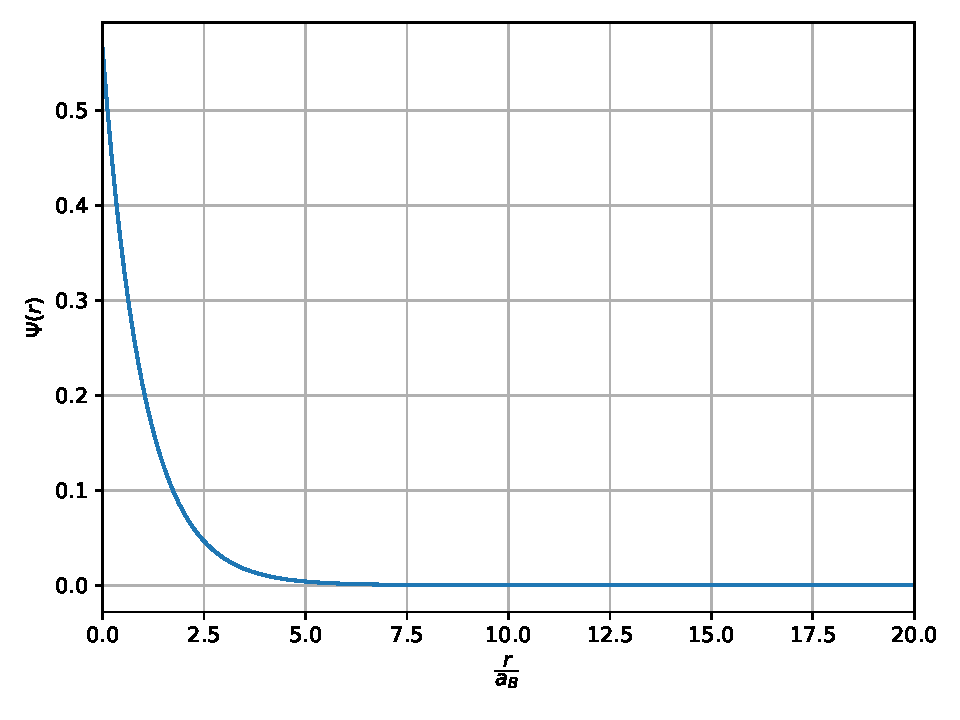
\includegraphics{Graph_a.pdf}
    \caption{Ausgeleichsfunktion zur Bestimmung des Absorptionskoeffizienten.}
    \label{fig:plot1}
  \end{figure}

Aus der Ausgleichsrechung wird der Absorptionskoeffizienten 
\begin{equation*}
    \sigma =  \left( 96.958 \pm 5.079 \right) \mathbin{/} \unit{\meter}
\end{equation*}

abgelesen. Die Anfangsaktvität bzw. der y-Achsenabschnitt, ist mit 
\begin{equation*}
    \text{A} =  \left( 111.434 \pm 1.024 \right)  \dfrac{1}{\unit{\second}}
\end{equation*}
gegeben.